\documentclass[11pt,a4paper]{article}
\usepackage[utf8]{inputenc}
\usepackage[T1]{fontenc}
\usepackage{amsmath,amssymb}
\usepackage{graphicx}
\usepackage{hyperref}
\usepackage{booktabs}

\title{Notes on the Harmonic Oscillator in Phase Space}
\author{A. Prism User}
\date{October 2026}

\begin{document}
\maketitle

\begin{abstract}
These notes collect the standard results on the quantum harmonic oscillator
and compare them with the classical phase-space picture~\cite{sakurai2017,griffiths2018}.
\end{abstract}

\section{Introduction}
The harmonic oscillator is the first system every course solves twice: once with
differential equations and once with ladder operators~\cite{dirac1958}.

\section{Ladder operators}
Define the annihilation operator
\begin{equation}
  a = \sqrt{\frac{m\omega}{2\hbar}}\left(x + \frac{i p}{m\omega}\right),
  \label{eq:a}
\end{equation}
so that the Hamiltonian becomes
\begin{equation}
  H = \hbar\omega\left(a^\dagger a + \tfrac{1}{2}\right).
  \label{eq:H}
\end{equation}
The commutator $[a, a^\dagger] = 1$ follows from $[x,p]=i\hbar$.

\subsection{Spectrum}
The energies are $E_n = \hbar\omega(n + \tfrac12)$, and the ground state
satisfies $a\,\psi_0 = 0$, which gives
\begin{equation}
  \psi_0(x) = \left(\frac{m\omega}{\pi\hbar}\right)^{1/4} e^{-m\omega x^2/2\hbar}.
  \label{eq:psi0}
\end{equation}

\section{Phase-space picture}
Figure~\ref{fig:ellipse} shows the classical trajectory as an ellipse whose area
grows with the energy, matching the Bohr--Sommerfeld rule~\cite{griffiths2018}.
\begin{figure}[htbp]
  \centering
  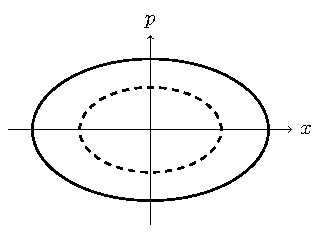
\includegraphics[width=0.5\linewidth]{figures/ellipse.pdf}
  \caption{Classical phase-space orbit of the oscillator.}
  \label{fig:ellipse}
\end{figure}

\begin{table}[htbp]
  \centering
  \begin{tabular}{@{}lcc@{}}
    \toprule
    Level & Energy & Parity \\
    \midrule
    $n=0$ & $\tfrac12\hbar\omega$ & even \\
    $n=1$ & $\tfrac32\hbar\omega$ & odd \\
    \bottomrule
  \end{tabular}
  \caption{The two lowest levels.}
\end{table}

\section{Conclusion}
Equations~\eqref{eq:a}--\eqref{eq:psi0} are all one needs for most applications.

\bibliographystyle{plain}
\bibliography{refs}
\end{document}
